% Part 4 implementation report draft (VGTC template style)

\documentclass{vgtc}                          % final (conference style)
% \documentclass[review]{vgtc}                % review
%\documentclass[widereview]{vgtc}             % wide-spaced review
%\documentclass[preprint]{vgtc}               % preprint
%\documentclass[electronic]{vgtc}             % electronic version

\graphicspath{{figures/}{pictures/}{images/}{./}}

\usepackage{times}
\renewcommand*\ttdefault{txtt}
\usepackage{mathptmx}

% Minimal packages for compact layout
\usepackage{enumitem}

\onlineid{0}
\vgtccategory{Research}
\vgtcinsertpkg

\title{PitchLens: A Workflow-Centered Visual Analytics Tool for Soccer Tactical Analysis}

\author{Wentao Mou\thanks{e-mail: wmou6@gatech.edu}\\ %
        \scriptsize Georgia Institute of Technology}

\abstract{
Soccer clubs increasingly rely on event logs and, when available, positional data for match review, opponent scouting, and player evaluation. In practice, the workflow remains fragmented across video tools, dashboards, and ad-hoc scripts, making it difficult to connect broad tactical observations to concrete possessions and moments. This report presents the current implementation of \textbf{PitchLens}, a workflow-centered visual analytics prototype for soccer tactical analysis. PitchLens is implemented as an event-first, dashboard-style system that allows analysts to (1) filter possessions under explicit context constraints, (2) inspect summary signals, (3) retrieve representative possessions with interpretable ranking reasons, (4) compare matched possession sets side-by-side, and (5) export an evidence-backed tactical note. The current Part 4 implementation demonstrates the feasibility of the proposed research idea and completes the core interactive loop, while richer evaluation, interface cleanup, and additional polish remain future work.
}

\keywords{Soccer; sports analytics; visual analytics; spatiotemporal visualization; tactical analysis; comparative analysis.}

\begin{document}
\firstsection{Introduction}
\maketitle

\noindent\textbf{Q1. What are you trying to do?}\\
I want to build one tool that helps me turn a broad idea about how a team plays into a short list of specific examples from real matches that clearly show the idea. I also want the tool to let me compare those examples across two opponents or two matches under the same match conditions, so the comparison is fair. My goal is to make it fast to answer: ``What is the pattern, where are the examples, and how does it differ across opponents?''

\noindent\textbf{Q2. How is it done today, and what are the limits of current practice?}\\
In current practice, people usually rely on several tools, each good at one part of the analysis, and then piece the results together to answer a full question. Prior work has shown tools that help with different parts of the job, such as tracking how a team’s shape changes over time \cite{Wu2019ForVizor}, understanding how the ball moves through passes \cite{Xie2021PassVizor}, comparing possible lineups \cite{Cao2023TeamBuilder}, interpreting important moments in context \cite{Cao2024ActionEvaluator}, and exploring scouting scenarios \cite{Cao2025TeamScouter}. Other work also shows that it helps when a tool can connect summaries back to the exact moments in a match and even link back to video \cite{Stein2018BringItToThePitch}. Public datasets have also made it easier to build and test tools without special access \cite{Pappalardo2019SoccerLogs,Bassek2025BundesligaDataset}. Despite this progress, two limits remain common. First, it is still slow to go from a summary to a short, convincing set of example possessions. Second, comparisons across opponents or matches are fragile because they depend on manually matching the same match situations; small mismatches can change the conclusion.

\noindent\textbf{Q3. What is new in your approach and why do you think it will be successful?}

I propose \textbf{PitchLens} (working title), a New Domain Tool designed around a simple evidence loop: start from a broad observation, retrieve representative possessions, and compare those possessions under the same explicit game situations. The novelty is not a new visual form; it is treating evidence retrieval and fair comparison as central requirements rather than add-on features. I expect this approach to work because prior research already validates the usefulness of each analysis lens independently and shows that analysts benefit when summaries are grounded in concrete, replayable evidence \cite{Wu2019ForVizor,Xie2021PassVizor,Cao2024ActionEvaluator,Stein2018BringItToThePitch}. PitchLens focuses on reducing the practical cost of moving from a claim to the specific possessions that support it, while keeping comparison conditions visible and consistent.

\noindent\textbf{Q4. Who cares? If you are successful, what difference will it make?}\\
If I succeed, analysts and coaches should be able to produce faster and more defensible scouting and review reports, because every claim can be backed by a small set of example possessions and those examples can be compared under the same conditions. This matters because tactical decisions are time-sensitive and routinely debated. From a visualization perspective, PitchLens would contribute design knowledge about how to build domain tools that prioritize evidence retrieval and robust comparison, consistent with established guidance for design studies and evaluation \cite{Sedlmair2012DesignStudy,Munzner2009NestedModel,McKenna2014DesignActivity,Lam2012Evaluation}.

\section{Related Work}
I structure the literature review into three sub-directions: (1) soccer
visual analytics systems, (2) soccer data foundations and action valuation,
and (3) general visualization techniques for comparison and coordinated analysis
that inform my design. I emphasize not only what each line of work contributes,
but also what it leaves open for a workflow-centered integration.

\subsection{Soccer Visual Analytics Systems}
Soccer visual analytics has produced domain tools tailored to specific tasks and
representations, often with careful design grounded in analyst needs. ForVizor
characterizes formation evolution over phases to help explain how and why
formations change \cite{Wu2019ForVizor}. This work motivates my emphasis on
formation as a first-class analytic context rather than a static label: the same
passing network can reflect very different intentions depending on formation
dynamics and phase transitions. PassVizor focuses on passing dynamics and
supports detecting changes in passing tactics through interactive exploration and
drill-down \cite{Xie2021PassVizor}. I take from PassVizor the importance of
connecting overview summaries to concrete passing processes; however, I aim to
broaden the linking so that passing findings are immediately interpretable
alongside formation evolution and downstream outcomes.

More recent soccer VA systems broaden the scope of supported decisions.
Team-Builder addresses lineup selection by enabling multi-factor comparison and
explanation for coaching decisions \cite{Cao2023TeamBuilder}. This highlights that
soccer decisions are multi-criteria and that analysts need comparison interfaces
that avoid collapsing everything into a single score. Action-Evaluator targets
action-level player evaluation and emphasizes contextual interpretation rather
than isolated scores \cite{Cao2024ActionEvaluator}, which aligns with my focus on
evidence-based explanation. Team-Scouter extends the pipeline to scouting via
simulation-based what-if analysis for assessing player fit \cite{Cao2025TeamScouter}.
While my proposal does not aim to replicate simulation, Team-Scouter reinforces
the importance of comparison across scenarios and of making assumptions explicit
when supporting decision-making.

A recurring theme across these systems is that analysts need to move repeatedly
between \emph{signals} (summaries, rankings, model outputs) and \emph{evidence}
(concrete possessions and moments). This pattern appears explicitly in systems
that support narrative construction or communication. SoccerStories, for example,
was an early system that highlighted how interactive views can support visual
storytelling for soccer analysis and presentation \cite{Perin2013SoccerStories}.
This idea matters for PitchLens because practical analysis outputs are often
shared with coaches and players; a tool that cannot quickly produce interpretable
evidence (clips/possessions) often fails to influence decisions.

Earlier work on feature-driven visual analytics demonstrates how tracking-derived
movement features can be explored across player and team levels \cite{Janetzko2014VASTSoccer}.
I interpret this as a general lesson: analysts need multi-level navigation
(overview to detail) and the ability to reconcile alternative explanations by
inspecting evidence at different granularities. Finally, Bring It to the Pitch
provides evidence that combining video and movement data can strengthen analysis
by grounding patterns in the original footage \cite{Stein2018BringItToThePitch}.
Even if I start with event-first data, I treat the principle as design guidance:
my system should always make it easy to move from an abstract claim to replayable
evidence (possessions, spatial replays, and optionally video). More broadly, sports
visualization work has emphasized that domain tools must be anchored in real tasks,
iterative design, and actionable outputs rather than isolated charts
\cite{Aigner2011SportsVis,Santos2018VisualPerformance}.

\textbf{Implication for my gap.}
Collectively, these systems validate soccer as a strong application area and provide
high-quality designs for specialized tasks. However, many tools emphasize one focal
lens (formation, passing, lineup, or action evaluation). My proposal targets the
integration space between these lenses: I aim to reduce the cost of shifting between
representations and to make comparisons and explanations consistent across the workflow.
In practice, this means my related work is not ``missing a view,'' but ``missing an
end-to-end linking strategy'' that makes tactical narratives traceable and comparisons fair.

\subsection{Data Foundations and Action Valuation}
Tool capabilities depend on accessible, reliable data and interpretable derived measures.
Public event datasets enable reproducible analysis at scale and make event-first prototyping
realistic \cite{Pappalardo2019SoccerLogs}. For my scope, this is important: I can build a
useful prototype without privileged access, and I can frame the system around possessions,
sequences, and context filters that are available from events alone. Integrated datasets
combining event and tracking data reduce friction for multi-modal analysis and support richer
spatial reasoning \cite{Bassek2025BundesligaDataset}. I treat these datasets as an extension
path: they enable formation snapshots from positions and allow more precise notions of
pressure and spacing, but the core workflow (comparison and traceability) should already
function with events. Broader surveys of spatiotemporal team-sport analysis discuss common data
representations, tasks, and challenges, motivating treating possessions and transitions as
first-class objects \cite{Gudmundsson2017SpatioTemporal,Rein2021SportsData}.

Action valuation offers a principled way to quantify contributions beyond goals. VAEP-style
frameworks value actions via changes in short-term scoring and conceding probabilities
\cite{Decroos2018VAEP,Decroos2020VAEP_IJCAI}. For my proposal, action value is useful because it
produces a ranked set of influential moments that can serve as entry points for explanation;
however, it also introduces the risk of over-trusting a model score. The relevant design
question is therefore not ``how do I compute a better value model?'' but ``how do I present
value so it remains interpretable and evidence-backed?'' This motivates my plan to treat action
value as retrieval and explanation scaffolding: I want users to click a high-value action and
immediately see the possession context, the spatial situation, and comparable examples under
similar contexts, rather than consuming the number as an opaque truth.

In addition to action valuation, applied soccer analytics has popularized probability-based
measures such as expected goals (xG) to contextualize shot quality and to prioritize moments
for review; these measures are useful precisely because they help analysts focus attention, but
they still require concrete evidence when used in decision discussions \cite{Spearman2018BeyondGoals}.
Work that assesses team strategy from spatiotemporal data similarly motivates examining repeatable
patterns across possessions and relating them to outcomes \cite{Lucey2013Quality}. These perspectives
support the core workflow requirement in PitchLens: prioritization signals are most valuable when they
lead directly to representative possessions that can be inspected and compared.

\textbf{Implication for my gap.}
Existing datasets and valuation methods make it feasible to build and evaluate an integrated tool
within 1--2 semesters. The remaining challenge is interface-level: connecting derived metrics to
tactical reasoning without losing interpretability. This supports my focus on coordinated views and
traceable sequence retrieval.

\subsection{Comparison and Coordinated Analysis Techniques}
Soccer workflows are inherently comparative (opponent vs.\ opponent, match vs.\ match, phase vs.\ phase,
player vs.\ player). General visualization research provides reusable patterns for scalable comparison
and coordinated views, which I plan to adapt rather than inventing entirely new encodings.

NodeTrix illustrates hybrid representations balancing global structure and dense local inspection
\cite{Henry2007NodeTrix}. I see this as relevant to passing structure, where analysts may want both a
global view of connectivity and a detailed view of dense substructures (e.g., triangles in a build-up channel).
UpSet supports scalable set-intersection reasoning \cite{Lex2014UpSet}, which suggests a way to summarize
co-occurring tactical conditions and to keep comparisons explicit (e.g., which possessions match both a
formation state and a pressure condition). LineUp supports multi-attribute ranking and comparison
\cite{Gratzl2013LineUp}, which is relevant for soccer because analysts rarely decide based on one metric;
instead, they trade off progression, risk, value, and stability. MatrixWave demonstrates matrix-based visual
comparison of event sequences \cite{Zhao2015MatrixWave}. I view this as conceptually aligned with comparing
possession chains: even if the exact encoding differs, the key idea is to support side-by-side reasoning about
patterns in sequences rather than relying on isolated aggregate counts.

Sequence-focused techniques further motivate treating possessions as comparable objects. EventFlow demonstrates
how interactive filtering and aggregation can support analysis of temporal event sequences and retrieval of
concrete instances that match a pattern \cite{Plaisant2013EventFlow}. This is closely aligned with my design
goal of evidence-first drill-down: I want any overview to yield representative possessions quickly.

Because PitchLens is a domain tool contribution, methodology and evaluation guidance also form part of the
relevant state-of-the-art. Design study methodology describes how to identify domain needs, iterate designs with
stakeholders, and report transferable design knowledge \cite{Sedlmair2012DesignStudy,McKenna2014DesignActivity}.
Munzner’s nested model provides a structured way to reason about validity across the problem, data/operations,
encoding/interaction, and algorithm levels \cite{Munzner2009NestedModel}. Empirical evaluation work clarifies
trade-offs among study types and what evidence they provide \cite{Lam2012Evaluation}. These frameworks guide how
I will validate whether PitchLens improves traceability and comparison in realistic soccer analysis tasks.

\textbf{Implication for my gap.}
These technique and methodology papers suggest that my contribution should emphasize workflow and coordination
rather than a single novel encoding. I aim to combine (i) explicit context control for fair comparisons,
(ii) coordinated summaries across formation, passing, and value, and (iii) traceable drill-down to possessions.
My novelty claim is therefore centered on an integrated, evidence-driven workflow for soccer tactical narratives,
grounded in and distinguished from existing soccer VA systems and general comparative visualization techniques.

% ===================== Method & Plan =====================
\section{Method \& Plan}

\subsection{Contribution Type and Design Goals}
PitchLens is best framed as a \textbf{Design Study} contribution. The main goal is to build a working, interactive, dashboard-like visualization system for soccer tactical analysis rather than a standalone novel encoding or algorithm. The core system goal is to turn an analyst's high-level tactical claim into a compact, inspectable, and comparable evidence set. I focus on three design goals:

\begin{itemize}[leftmargin=*]
\item \textbf{G1 (Traceability):} Every summary-level claim should link to concrete possessions and moments.
\item \textbf{G2 (Fair Comparison):} Cross-match or cross-opponent comparisons should be made under explicit and matched context constraints.
\item \textbf{G3 (Workflow Efficiency):} The full loop from signal discovery to evidence package should be fast enough for real analysis practice.
\end{itemize}

This scope follows design-study principles for domain tools: anchor the system in real tasks, keep assumptions explicit, and evaluate whether the tool supports defensible reasoning in practice \cite{Sedlmair2012DesignStudy,Munzner2009NestedModel}. It also matches the expected deliverable for a design-study style class project: a generally runnable interactive visualization system, even if some advanced features and polish remain incomplete.

\subsection{Method: Evidence-Centered Workflow}
PitchLens implements a three-stage workflow:

\begin{enumerate}[leftmargin=*]
\item \textbf{Signal discovery.} The analyst first selects context (opponent, phase, score state, time window, field zone), then inspects summaries (formation tendency, passing progression, action value distribution).
\item \textbf{Evidence retrieval.} After selecting a signal, the system retrieves representative possessions that best support the selected pattern.
\item \textbf{Fair comparison.} The analyst compares two possession sets under the same explicit constraints and inspects where patterns diverge.
\end{enumerate}

\noindent\textbf{Core data objects.}
I model the analysis around possessions (not single events). Each possession stores:
(i) event sequence,
(ii) context tags (phase, zone, score state, transition type),
(iii) derived descriptors (progression, pressure proxy, action value summaries).

\noindent\textbf{Retrieval ranking.}
For each candidate possession $p$, I use an interpretable weighted score:
\[
S(p)=\alpha R_{\mathrm{signal}}(p)+\beta R_{\mathrm{context}}(p)+\gamma R_{\mathrm{diversity}}(p), \quad
\alpha+\beta+\gamma=1.
\]
$R_{\mathrm{signal}}$ captures relevance to the selected tactical signal, $R_{\mathrm{context}}$ measures match quality to user-defined constraints, and $R_{\mathrm{diversity}}$ reduces near-duplicate examples in the returned set.

\subsection{System Design and Current Prototype}
The current prototype centers on four coordinated views:

\begin{itemize}[leftmargin=*]
\item \textbf{V1: Context Filter Panel} (opponent, game state, phase, zone, time).
\item \textbf{V2: Pattern Summary View} (overview signals for quick hypothesis formation).
\item \textbf{V3: Possession Retrieval View} (ranked representative possessions with why-selected metadata).
\item \textbf{V4: Comparison Workspace} (side-by-side matched sets with synchronized inspection).
\end{itemize}

\begin{figure}[t]
\centering
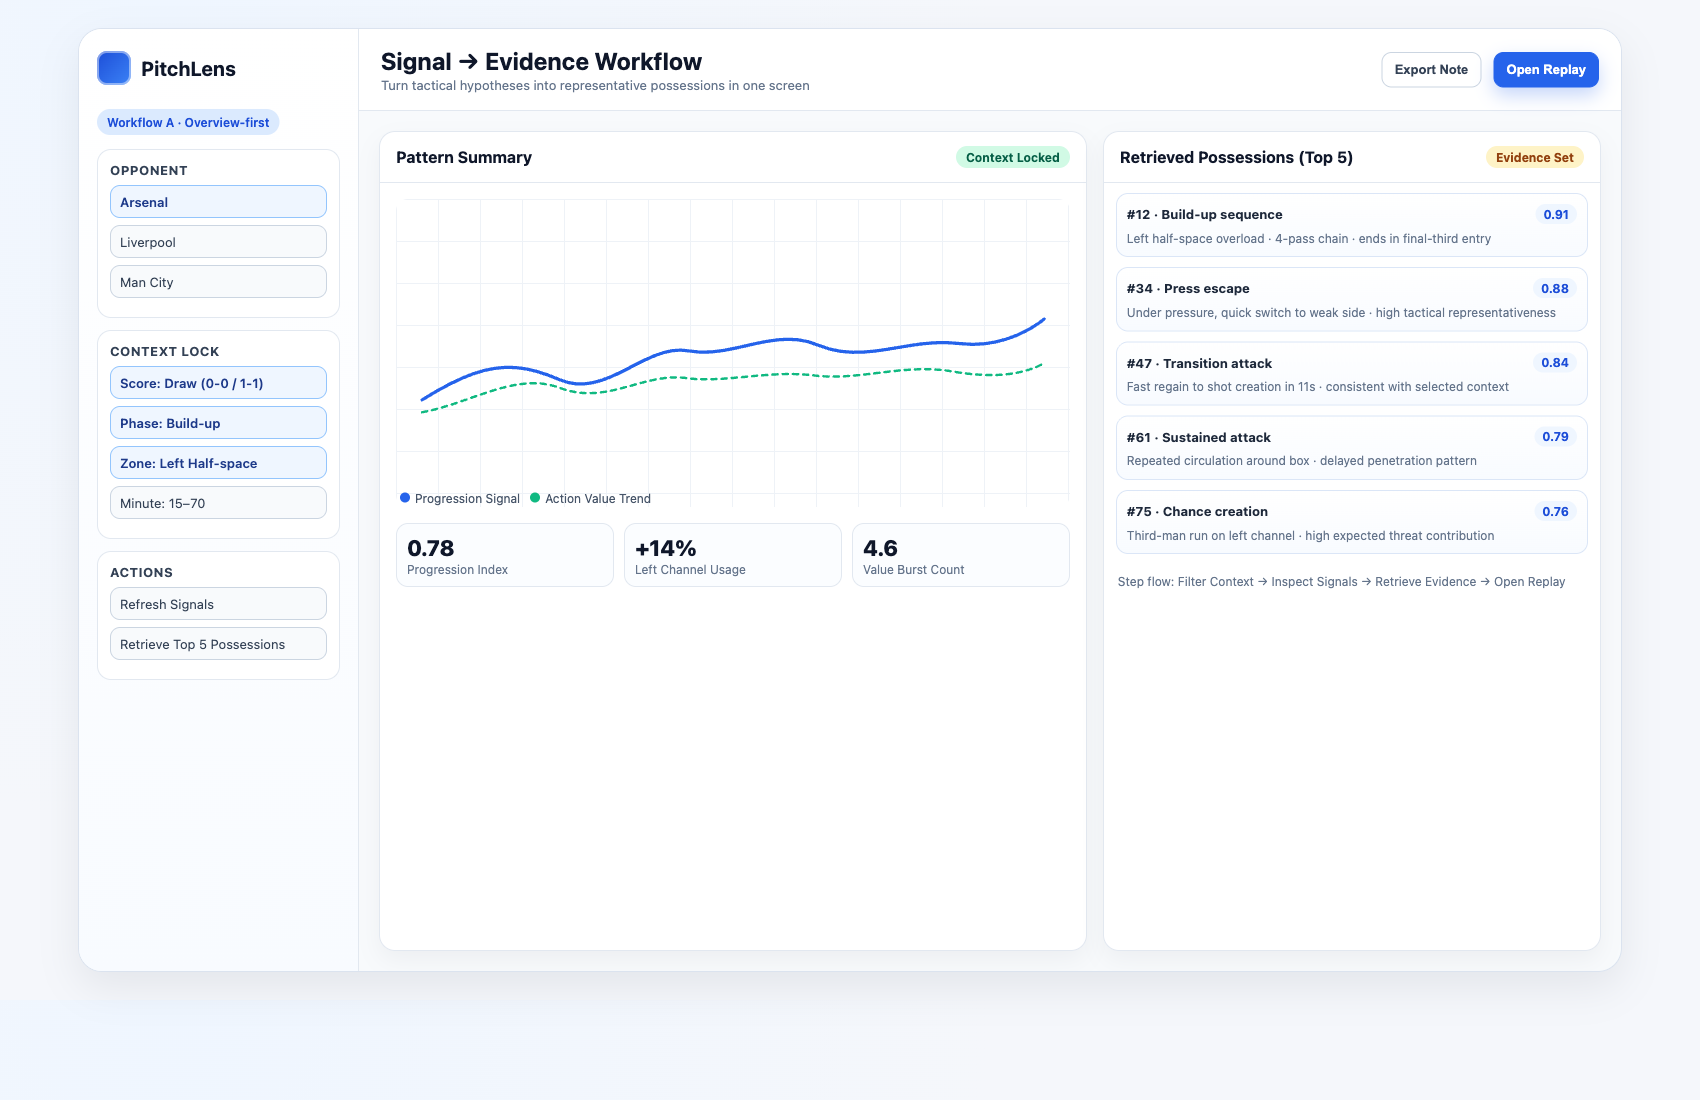
\includegraphics[width=\columnwidth]{figures/sketch_a_figma.png}
\caption{PitchLens overview-first interface: analysts filter context, inspect summary signals, and retrieve representative possessions.}
\label{fig:pitchlens_mockup_a}
\end{figure}

\begin{figure}[t]
\centering
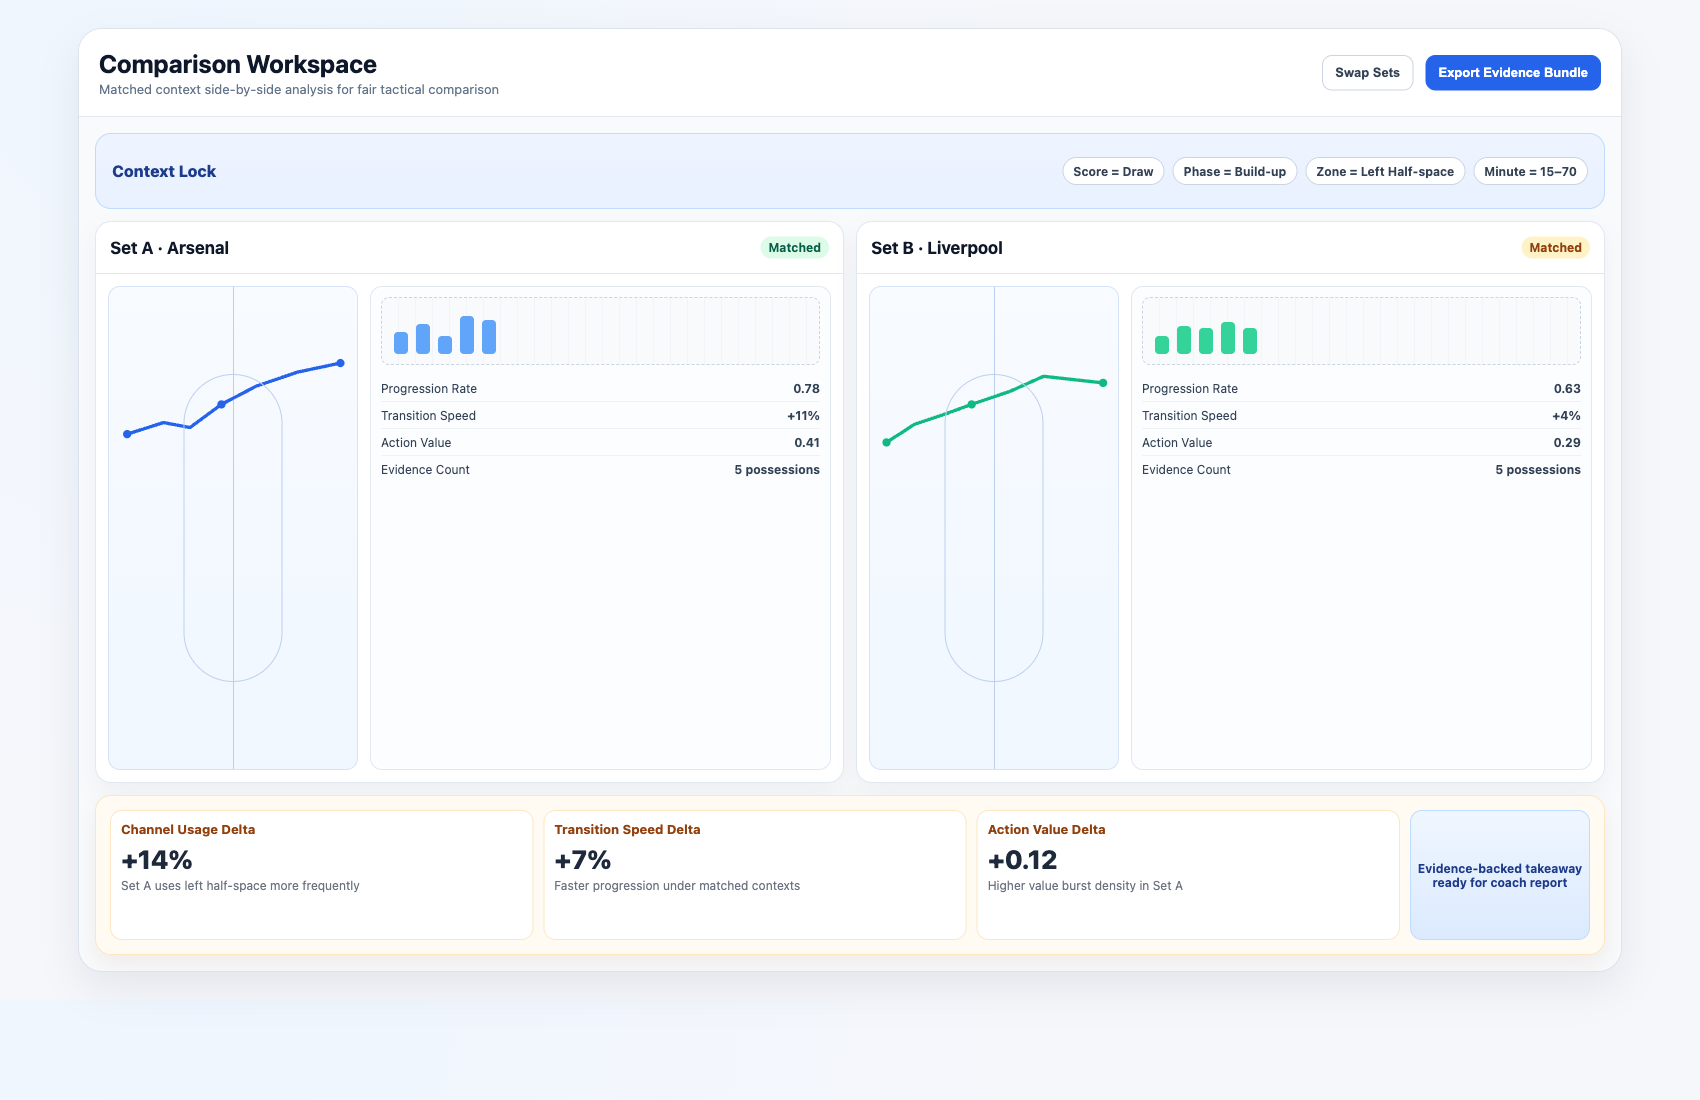
\includegraphics[width=\columnwidth]{figures/sketch_b_figma.png}
\caption{PitchLens comparison workspace: two matched possession sets are compared under explicit context lock with interpretable deltas.}
\label{fig:pitchlens_mockup_b}
\end{figure}

\noindent
These sketches informed the current implementation. In the running prototype, the system now supports a complete event-first analysis loop across filtering, summary inspection, representative retrieval, comparison, and export. The visual design is still being refined, but the interaction structure shown in the sketches has been translated into a functional local web application.

\subsection{Current Implementation and Part 4 Progress}
\noindent\textbf{Implementation strategy.}
To keep the system feasible within one semester, I implemented PitchLens as an event-first prototype. The current system is built as a local web application with a lightweight frontend and data-processing pipeline, and it runs from either synthetic sample data or imported structured match data. I also added a free public-data path using StatsBomb Open Data so the prototype can be demonstrated on real matches without requiring a paid provider.

\noindent\textbf{Implemented core pipeline.}
The current implementation includes:
\begin{itemize}[leftmargin=*]
\item event ingestion from local CSV/JSON files and a free StatsBomb Open Data adapter,
\item possession normalization/segmentation and context tagging,
\item descriptor extraction for progression, lane, pass count, turnover-before-midline, and success-to-middle-third,
\item interpretable representative retrieval using the weighted score defined above,
\item side-by-side fair comparison under explicit shared filters,
\item markdown export for evidence-backed tactical notes.
\end{itemize}

\noindent\textbf{Implemented interactive functionality.}
The running prototype already supports the main analysis workflow expected for this project:
\begin{itemize}[leftmargin=*]
\item explicit context filters over opponent, score state, phase, time window, minute range, and start zone,
\item at least four summary metrics/signals, including lane share, average progression distance, passes before middle-third access, turnover-before-midline rate, and success-to-middle-third rate,
\item representative possession retrieval with why-selected explanations,
\item matched side-by-side comparison with interpretable deltas,
\item export of a short tactical note grounded in retrieved evidence.
\end{itemize}

\noindent\textbf{Current Part 4 status.}
For this Part 4 submission, I consider the project to be roughly \textbf{60\% complete}. The core visuals, data pipeline, and interaction loop are functional and runnable, which satisfies the main implementation goal for this stage. What remains incomplete is the final polish: cleaner UI refinement, more systematic evaluation, stronger reporting around results, and tighter integration of optional extensions such as direct video linkage and assistant-style support. These extensions exist in prototype form in the codebase, but they are secondary to the core event-first workflow and are not required for the main deliverable.

\noindent\textbf{Implementation boundaries.}
I intentionally kept the prototype focused on traceability and interpretability instead of attempting a fully automated broadcast-analysis system. This means the current version is strong enough to demonstrate feasibility and support realistic analysis tasks, but it is still a research prototype rather than a finished production tool. This tradeoff is consistent with the course expectation that a Part 4 implementation should be ambitious but not fully polished.

\subsection{Current Validation and Remaining Evaluation}
For Part 4, I focus on demonstrating that the system is runnable, that the core workflow can be completed end-to-end, and that the implemented interactions support the intended analysis tasks. This level of validation is appropriate for a design-study style prototype at roughly 60\% completion \cite{Lam2012Evaluation,Sedlmair2012DesignStudy}. The current validation therefore emphasizes implementation feasibility, workflow coverage, and traceability rather than a full summative user study.

\noindent\textbf{Current validation focus.}
\begin{itemize}[leftmargin=*]
\item \textbf{Runnable prototype:} the codebase is executable locally with the provided code, data, and adapters.
\item \textbf{Workflow coverage:} the system already supports the full event-first loop from context filtering to exported tactical note.
\item \textbf{Interpretability:} ranking reasons, explicit context constraints, and comparison deltas remain visible during analysis.
\item \textbf{Real-data feasibility:} the prototype can run on synthetic sample data and on free public match data through the StatsBomb Open Data adapter.
\end{itemize}

\noindent\textbf{Remaining evaluation plan.}
After Part 4, I plan to run a task-based study with analysts or advanced students familiar with soccer event analysis, following guidance on empirical evaluation scenarios \cite{Lam2012Evaluation}.

\noindent\textbf{Planned study conditions.}
\begin{itemize}[leftmargin=*]
\item \textbf{C0 (Baseline):} Fragmented workflow (separate dashboards/manual search).
\item \textbf{C1 (PitchLens):} Integrated evidence-centered workflow.
\end{itemize}

\noindent\textbf{Planned study tasks.}
\begin{itemize}[leftmargin=*]
\item \textbf{T1:} Identify one tactical pattern for a target team in a selected match.
\item \textbf{T2:} Retrieve 3--5 representative possessions supporting that pattern.
\item \textbf{T3:} Compare the pattern across two opponents under matched context.
\item \textbf{T4:} Produce a short recommendation with linked evidence.
\end{itemize}

\noindent\textbf{Planned measures.}
\begin{itemize}[leftmargin=*]
\item \textbf{Objective:} task completion time, number of filter/query iterations, evidence coverage, comparison consistency.
\item \textbf{Subjective:} confidence in conclusions, perceived fairness of comparison, and SUS usability score.
\end{itemize}

\noindent\textbf{Planned hypotheses.}
\begin{itemize}[leftmargin=*]
\item \textbf{H1:} C1 reduces time from signal discovery to evidence package creation.
\item \textbf{H2:} C1 improves perceived fairness and consistency in cross-opponent comparison.
\item \textbf{H3:} C1 improves analyst confidence because claims remain linked to concrete possessions.
\end{itemize}

\subsection{Part 4 Deliverables and Remaining Work}
\begin{table}[t]
\centering
\small
\caption{Current Part 4 progress and remaining work.}
\label{tab:progress}
\begin{tabular}{p{0.16\linewidth}p{0.78\linewidth}}
\hline
Completed & Define the workflow-centered scope, review related work, and produce low-fidelity interface sketches. \\
Completed & Implement the event-first data pipeline, including possession normalization, context tagging, and descriptor extraction. \\
Completed & Implement the four coordinated views and the core loop for retrieval, comparison, and note export. \\
Completed & Add runnable sample data and a free public-data adapter so the system can be demonstrated out of the box. \\
In progress & Refine the interface, improve retrieval quality on more matches, and strengthen the clarity of exported evidence packages. \\
Remaining & Run a more formal task-based evaluation and incorporate findings into the final report and demo video. \\
\hline
\end{tabular}
\end{table}

\noindent\textbf{Primary deliverables.}
(1) a functional and runnable PitchLens prototype, (2) code and data or adapters needed to run the system out of the box, (3) an IEEE-format report with implementation details in the 3--4 page range excluding references, and (4) either evaluation results or an evaluation-ready plan plus design lessons for evidence-centered soccer VA.

\noindent\textbf{Main risks and mitigation.}
\begin{itemize}[leftmargin=*]
\item \textbf{R1:} Event-only context labels may be noisy. \textbf{Mitigation:} expose uncertainty and allow manual overrides.
\item \textbf{R2:} Retrieval may overfit one team style. \textbf{Mitigation:} test multiple matches/opponents and enforce diversity in retrieved sets.
\item \textbf{R3:} Users may over-trust ranking scores. \textbf{Mitigation:} show ranking factors and keep drill-down to replayable possessions one click away.
\end{itemize}
% =================== End Method & Plan ===================

\bibliographystyle{unsrt}
\bibliography{template}

\end{document}
